% CVPR 2022 Paper Template
% based on the CVPR template provided by Ming-Ming Cheng (https://github.com/MCG-NKU/CVPR_Template)
% modified and extended by Stefan Roth (stefan.roth@NOSPAMtu-darmstadt.de)

\documentclass[10pt,twocolumn,letterpaper]{article}

%%%%%%%%% PAPER TYPE  - PLEASE UPDATE FOR FINAL VERSION
% \usepackage[review]{cvpr}      % To produce the REVIEW version
% \usepackage{cvpr}              % To produce the CAMERA-READY version
\usepackage[pagenumbers]{cvpr} % To force page numbers, e.g. for an arXiv version

% Include other packages here, before hyperref.
\usepackage{graphicx}
\usepackage{amsmath}
\usepackage{amssymb}
\usepackage{booktabs}

% It is strongly recommended to use hyperref, especially for the review version.
% hyperref with option pagebackref eases the reviewers' job.
% Please disable hyperref *only* if you encounter grave issues, e.g. with the
% file validation for the camera-ready version.
%
% If you comment hyperref and then uncomment it, you should delete
% ReviewTempalte.aux before re-running LaTeX.
% (Or just hit 'q' on the first LaTeX run, let it finish, and you
%  should be clear).
\usepackage[pagebackref,breaklinks,colorlinks]{hyperref}


% Support for easy cross-referencing
\usepackage[capitalize]{cleveref}
\crefname{section}{Sec.}{Secs.}
\Crefname{section}{Section}{Sections}
\Crefname{table}{Table}{Tables}
\crefname{table}{Tab.}{Tabs.}


%%%%%%%%% PAPER ID  - PLEASE UPDATE
\def\cvprPaperID{0}
\def\confName{CSE 559a}
\def\confYear{2023}


\begin{document}

%%%%%%%%% TITLE - PLEASE UPDATE
\title{Project Proposal: Co-existing Object Conditioning for Open-Vocabulary Segmentation}

\author{
Tovi Tu \hspace{1in} Anthony Chen \hspace{1in} Shuhan(Steven) Zhang  \hspace{1in} Ben Mueller 
}
\maketitle

%%%%%%%%% ABSTRACT
\begin{abstract}
Semantic segmentation is essential in real world applications such as autonomous driving. However, Past models lack the flexibility to generalize to unseen objects common in the real-world setting. Recent developments in vision-language pretraining have shown incredible abilities to unify text and image encoders in a general embedding space with the potential to establish semantic correspondence between image and texts, enabling open-vocabulary semantic segmentation where a model assign pixel-wise class label beyond predefined categories. To exploit the latent distribution of co-occurring objects in a scene, this work propose to utilize a transformer-based model with a pretrained CLIP encoder and a ClipSeg decoder to segment images by predicting a sequence of object masks conditioned on previous outputs, expecting to achieve a better accuracy than the existing baseline method.

\end{abstract}

%%%%%%%%% BODY TEXT
\section{Project Overview}

\subsection{Motivation}

Semantic segmentation is a fundamental computer vision task being studied extensively in a fixed-category setting. However, past models with prediction heads trained in an end-to-end manner lack the flexibility to be readily applied to real-world scenarios since many categories missing in the training set are not recognizable. Recent advancements in image encoders supervised by natural language captions have demonstrated amazing abilities to learn cross-modal embeddings adaptable to various downstream tasks. The embedded semantic correspondence between image and text labels for a wide range of common objects can effectively extend the image classes beyond predetermined categories and allow for an easy adaptation to out-of-distribution data. 

\subsection{Problem Definition}

Open-vocabulary semantic segmentation falls into the category of zero-shot learning. This task challenges a model to assign pixel-level class labels from the set of all possible classes $C=C_{seen} \cup C_{unseen}$ to a given image $x\in X$, where $C_{seen}$ and $C_{unseen}$ are mutually exclusive sets and the former represents classes available in the training set $X_{train}$. The model is trained on $X_{train}$, with input images and ground truth annotation masks. During test time, the model is evaluated in a zero-shot setting, trying to correctly predict unseen labels $c\in C_{unseen}$ in addition to seen labels in the training set $X_{test}$. 

\subsection{Related Works}

A previous method, SimSeg \cite{simseg}, has successfully adapted pretrained CLIP models \cite{clip} for open-vocabulary segmentation by first predicting a class-agnostic mask and then classifying each masked image with CLIP. Since the vanilla CLIP model is trained to generate a global feature for any image, there is a granularity gap between the pretraining objective and the more fine-grained semantic segmentation objective. To close the gap, SimSeg complements MaskFormer \cite{maskformer}, a fixed-class segmentation model, with CLIP to extend the possible classes. However, it fails to exploit the relational information of objects present in the scene by categorizing one masked image at a time.

\subsection{Proposed Method}

Inspired by the distributional semantics theory, we propose to capture the distribution of co-existing objects in a scene. In a natural setting, objects in an image often appear together and collectively determine the overall context. Figure 1 gives an intuitive example. In the scenic shot, the appearance of a sea increases the probability of seeing a beach, and a hill is likely to be accompanied by clouds or the sky. The collection of the co-existing objects defines an abstract context of outdoor scenery and rules out the probability of seeing indoor concepts such as a sofa or a television. The latent prior distribution is potentially useful for detecting a set of objects in one image. 

Building upon the intuition, we propose a one-stage architecture that segments an object from the image auto-progressively by first targeting the most prominent object and then conditioning subsequent predictions on previous results. As a preliminary thought, we envision this model to have a transformer style and use a pretrained CLIP encoder and ClipSeg \cite{clipseg} decoder, a zero-shot semantic segmentation model conditioned on prompts, as the backbone. To adapt the prompt-conditioned model, We will modify the encoder for the support prompt so that it actively predicts the most probable object at the current timestep, which is different from those predicted in the previous timesteps. For the first prediction, we would condition the prediction on a learnable token to signify the start of the sequence and update it during training. Similar to the next token prediction language models, our model accepts a raw image and predicts a sequence of mutually exclusive masks with labels. We consider freezing those modules or fine-tuning them with a lower learning rate to avoid catastrophic forgetting in the backbone model.

\begin{figure} [h]
    \centering
    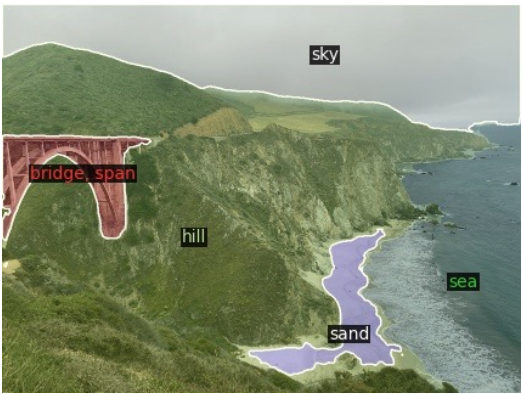
\includegraphics[width=0.5\linewidth]{images/seg_sample.png}
    \caption{Example Segmented Image from CLipSeg \cite{clipseg}}
    \label{fig:enter-label}
\end{figure}

\subsection{Goals}

We will evaluate the performance of our model on the same set of benchmarks as in \cite{simseg}. The minimum goal for this project is to implement a simple two-stage method similar to \cite{simseg} with a classifier and a mask generator but with the selected CLipSeg \cite{clipseg} backbone and evaluate its efficacy on one large-scale benchmark. If desirable performance is obtained, we will implement a unified model for both tasks and make meaningful use of the co-existing relations in images for prediction. We will experiment with different hyperprameters and training strategy to maximize the performance on a full-scale training dataset. For evaluation, we will benchmark the model on common segmentation datasets to compare the performance to other existing models. We expect our model to outperform the baseline.

\section{Team Member Roles/Tasks}
\label{sec:roles}
Following the structure for machine learning tasks, we have separated our overall project into 4 sections, data, architecture, training, and benchmark. Since some tasks are tightly coupled, such as data and benchmark, we will ensure communication among team members across sections to maintain alignment and efficiency. The detailed responsibility and assignment is outlined below:

\textbf{Tovi Tu - Architecture lead} is responsible for designing the overall structure of the models, including selecting the framework, algorithms, and methodologies. This is crucial and technically complex, which is why we assigned the task to our most technically familiar member in this field.


\textbf{Anthony Chen - Training lead} is responsible for developing and implementing the training procedure, optimizing model, and ensuring that the training is effective using the datasets. Since this involves more python familiarity and access to computational resources, this task is delegated to Anthony.


\textbf{Steven Zhang - Data lead} is responsible for researching, collecting, preprocessing, and augmenting datasets for the training procedures. This would require more research and data science expertise. 


\textbf{Ben Mueller - Benchmark lead} is responsible for running related work’s code on the predefined datasets to acquire benchmarks comparison, as well as running our model on multiple datasets to ensure quality and effectiveness. 



\section{Resources}
For computational resources, we will rely on personal NVIDIA 40 series graphics card's processing capabilities and have access to high-performance compute nodes including WashU Research Infrastructure \url{https://ris.wustl.edu/}, national research platform \url{https://nationalresearchplatform.org/} and other resources through our research labs. If necessary, we might also use Google Colab credits for extra computational power.

As the data plays an essential role, we will utilize the COCO stuff dataset\cite{cocostuff}, which provides detailed pixel-level annotations for a diverse array of objects and scenes, as shown in the figure. There are 118k training images labeled with 171 valid categories featuring common objects as the sky and cars. For evaluation, we will use the ADE20K \cite{ade20k} and Pascal VOC \cite{pascal} datasets to quantify the generalizability of the model.

For development, we plan to build upon the pretrained models and initialize the weights from open-source checkpoints accessible through huggingface \url{https://huggingface.co/docs/transformers/model_doc/clipseg}. We will also access the official codes for benchmark metric functions through the provided toolbox \url{https://github.com/CSAILVision/ADE20K}.

\begin{figure}[h]
    \centering
    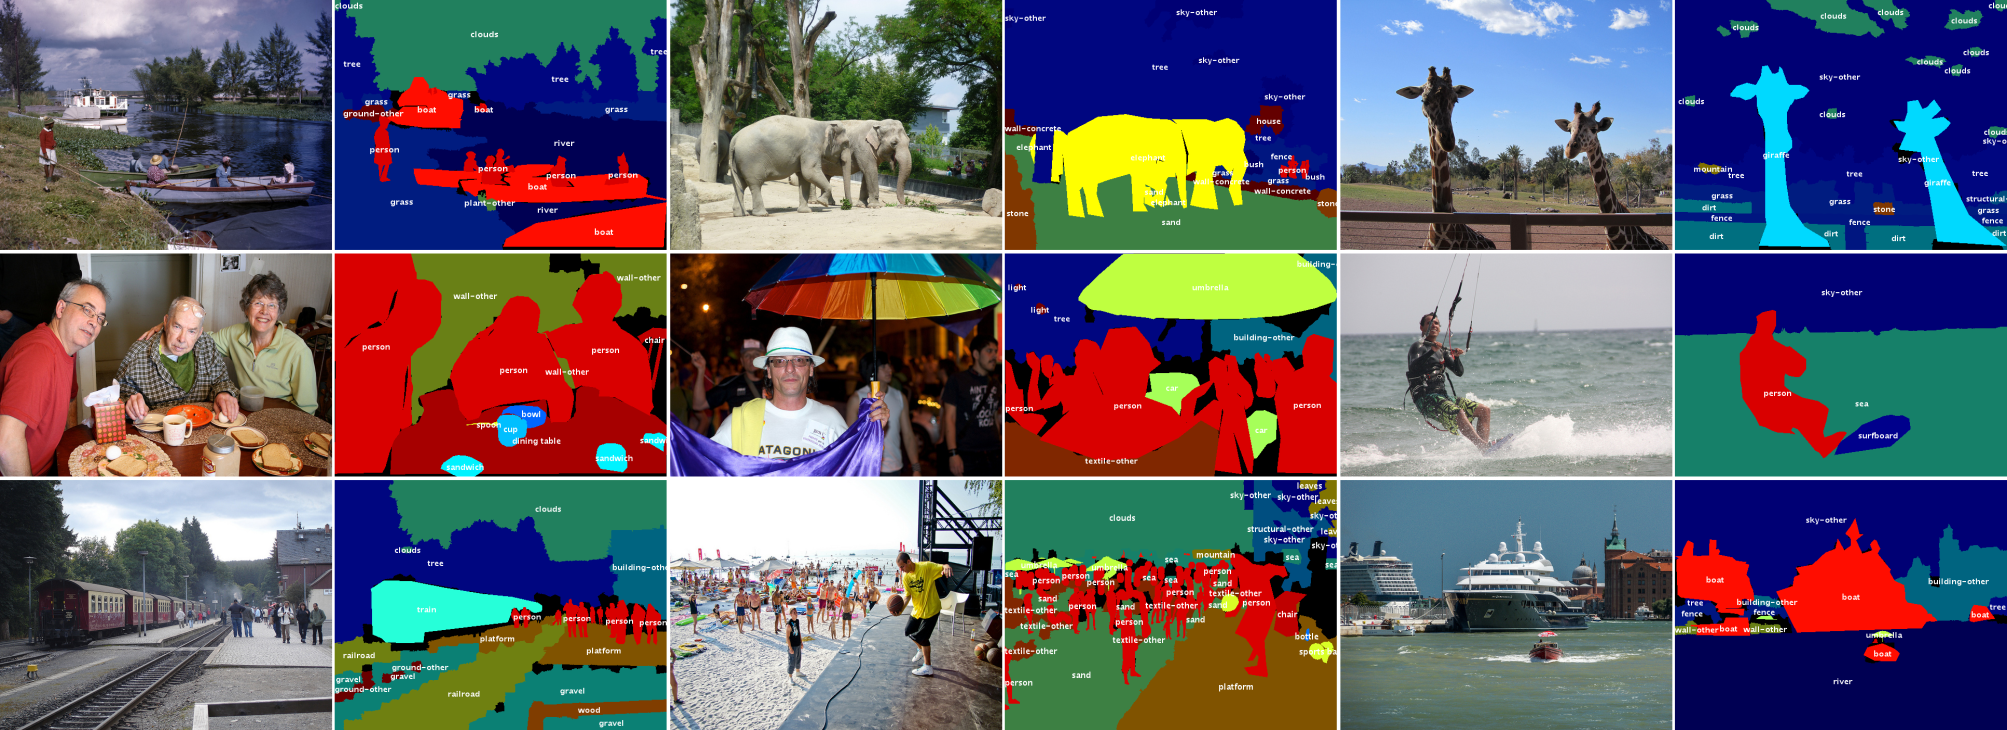
\includegraphics[width=0.9\linewidth]{cocostuff.png}
    \caption{Coco Stuff \cite{cocostuff} dataset with pixel-level annotations}
    \label{fig:enter-label}
\end{figure}

\section{Reservations}

One major reservation that we have with this project is that we won’t be able to fully anticipate the computational, training and testing, complexity until we perform further experimentation. As such, the datasets we plan to use may be too large for us to complete comprehensive training and benchmarking using the compute resources at our disposal. If this becomes a problem, we hope that for a minimal goal we will at least implement a object classifier and mask generator similar to \cite{simseg} and to be able to benchmark it on at least one of the common datasets. Another reservation is the lack of preliminary results to support the claimed method at the time of the proposal. Our hypothesis that relational knowledge of co-occurring objects may fall apart because such information may be intractable or contains too much noise for meaningful prediction.



\section{Relationship to Background}

\textbf{Tovi} is currently working on vision-language models under supervision of Prof. Chenguang Wang as an independent project with experience with machine learning and deep learning in time-series analysis and classification by using PyTorch and TensorFlow.

\textbf{Anthony} is taking NLP and CV, familiar with the ML training process. Currently working as a Tech Lead in an iOS application project from WashU medical school. Have more experiences on the tech side: code, GPU, data storing, interface.

\textbf{Steven} is experienced with pytorch and related frameworks. Moreover, through past independent research experiences in both WUSTL and Peking University, Steven is familiar with research methodologies related with image search tasks and the utilization CLIP. Steven is not quite familiar with deep learning, or the latest methodologies in computer vision.

\textbf{Ben} has experience training large scale models using pytorch and pytorch lightning in research settings, currently using these in a Bioinformatics/ML research project in the WashU medical school.



%%%%%%%%% REFERENCES
{\small
\bibliographystyle{ieee_fullname}
\bibliography{bibliography}
}

\end{document}
